\section{Experiments}
\label{sec:experiments}

\begin{table}[t]
\centering
\footnotesize
\setlength{\tabcolsep}{2.5pt}
\caption{Needle-in-a-Haystack accuracy (\%). Bold = best sparse method.}
\label{tab:niah}
\begin{tabular}{l|ccccc|ccccc}
\toprule
 & \multicolumn{5}{c|}{8K Context} & \multicolumn{5}{c}{32K Context} \\
 & 256 & 512 & 1K & 2K & 4K & 256 & 512 & 1K & 2K & 4K \\
\midrule
\multicolumn{11}{l}{\textit{Fast-dLLM 7B} (Exact: 100 / 88)} \\
Quest & \textbf{88} & 91 & 100 & 100 & 100 & 27 & 45 & \textbf{73} & \textbf{73} & \textbf{76} \\
Tidal & 85 & 67 & 76 & 82 & \textbf{100} & 12 & 27 & 27 & 27 & 61 \\
MAGE & 85 & \textbf{94} & \textbf{100} & \textbf{100} & \textbf{100} & \textbf{39} & \textbf{45} & 61 & 64 & 70 \\
\midrule
\multicolumn{11}{l}{\textit{Fast-dLLM 1.5B} (Exact: 100 / 91)} \\
Quest & 33 & \textbf{64} & 70 & 85 & 97 & 18 & 18 & 24 & 36 & \textbf{55} \\
Tidal & 21 & 42 & 67 & 82 & 97 & 12 & 15 & 18 & 24 & 33 \\
MAGE & \textbf{48} & 55 & \textbf{70} & \textbf{91} & \textbf{100} & \textbf{21} & \textbf{30} & \textbf{39} & \textbf{42} & 42 \\
\bottomrule
\end{tabular}
\end{table}


\begin{figure*}[t!]
    \centering
    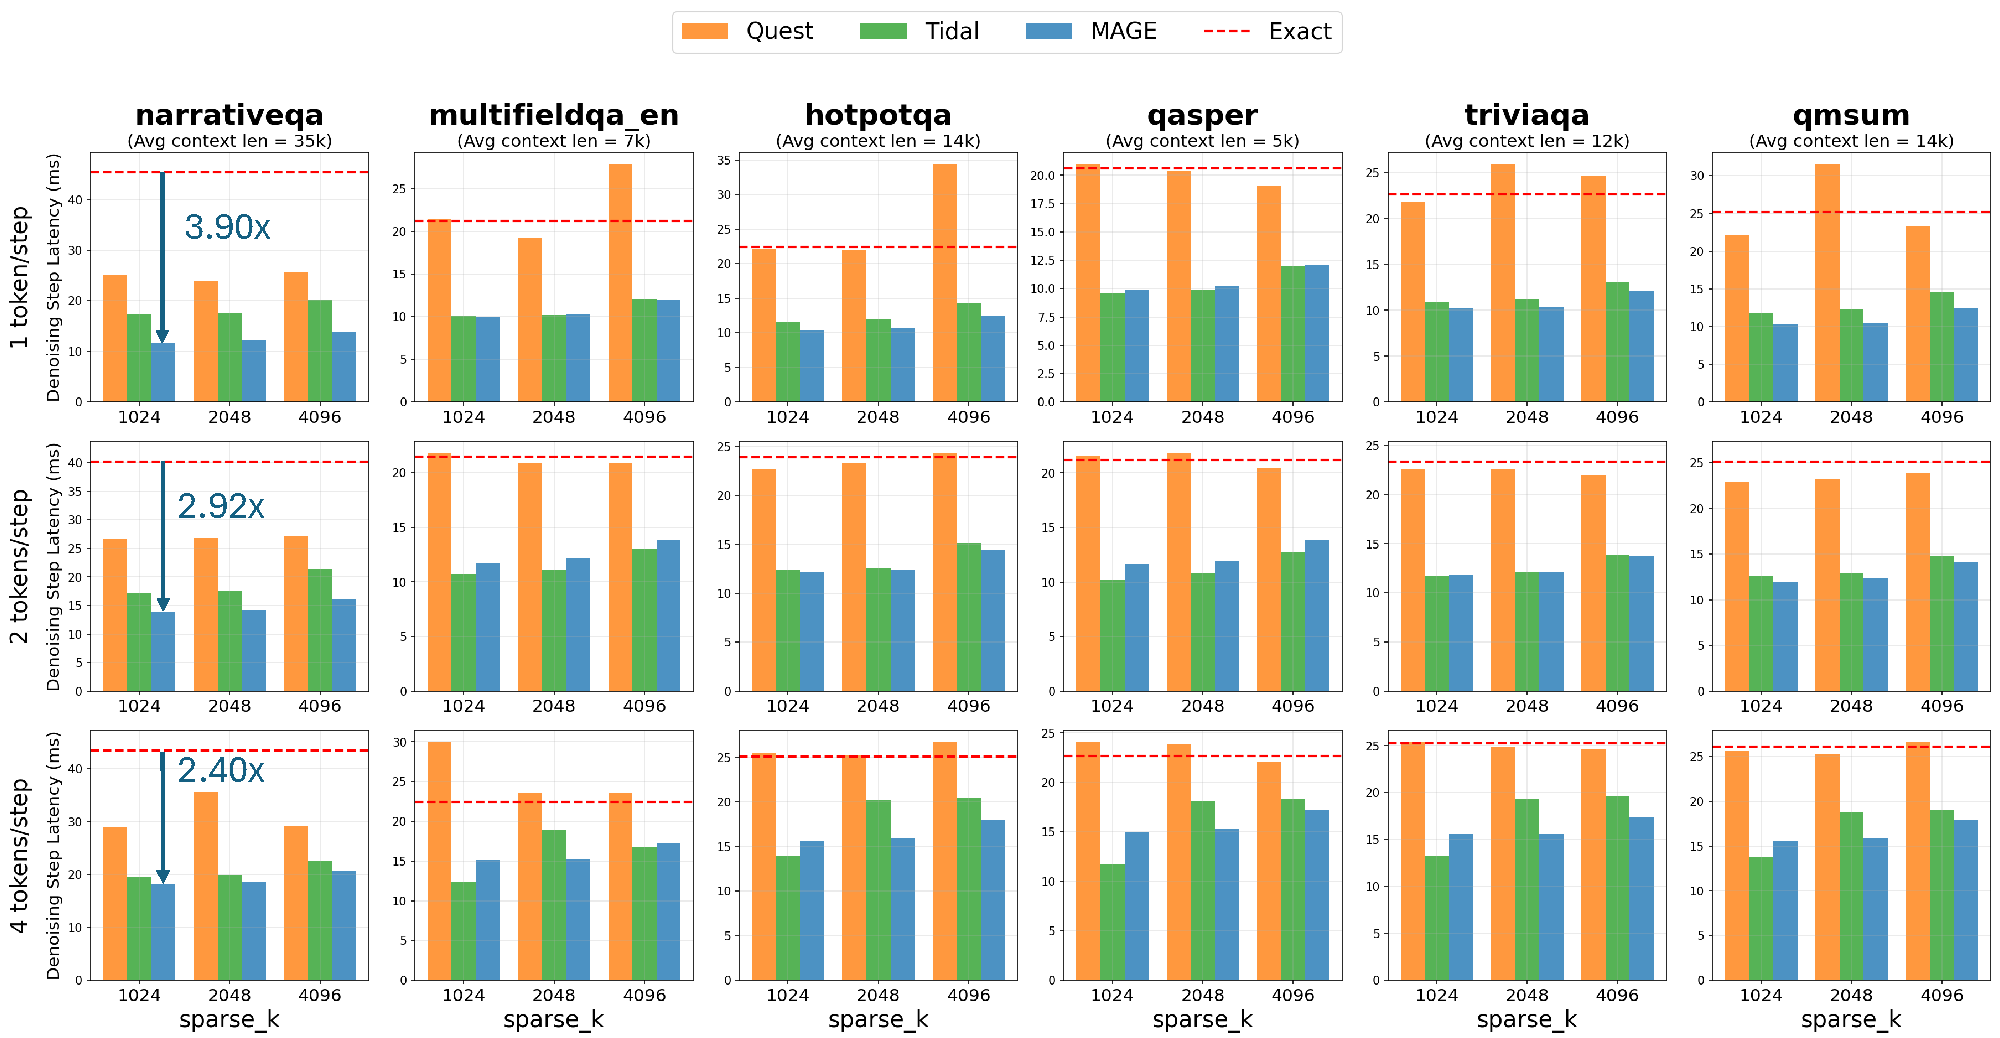
\includegraphics[width=\textwidth]{figures/fig6_avg_latency_per_step_1.5B.pdf}
    \caption{Per-task average denoising step latency on LongBench with Fast-dLLM 1.5B across three denoising configurations (1, 2, 4 tokens/step).}
    \label{fig:latency_1.5B}
\end{figure*}


\paragraph{Setup.}
We evaluate two variants of the proposed method: \textbf{MAGE} denotes the training-free version that directly leverages All-[\texttt{MASK}] block guidance , while \textbf{MAGE-FT} refers to the version further enhanced through our lightweight fine-tuning framework. We evaluate our methods on two different scale block diffusion models: Fast-dLLM 1.5B and Fast-dLLM 7B~\citep{wu2025fastdllmv2}. We compare our  methods against the exact attention method and two sparse attention methods: Quest~\citep{tang2024quest} and Tidal~\citep{yang2025tidaldecode}. 

We fine-tuned Fast-dLLM 1.5B and 7B for inference on a long-context subset from the Daring-Anteater dataset. Specifically, the 1.5B model was trained for 200 steps with a learning rate of $1 \times 10^{-5}$ and $\lambda=0.5$, while the 7B model used 100 steps, a learning rate of $5 \times 10^{-6}$, and $\lambda=1.5$, requiring only a few hours on a single NVIDIA H100 GPU. For unmasking, we use the static strategy to control the number of denoising steps and fairly compare the accuracy across all methods. All sparse attention kernels are implemented using FlashInfer~\citep{ye2025flashinfer}, and experiments are conducted on NVIDIA H100 GPUs.



\subsection{Accuracy Evaluation}
\label{subsec:accuracy}

\paragraph{LongBench.}
We evaluate on LongBench~\citep{bai2024longbenchbilingualmultitaskbenchmark}, a comprehensive long-context benchmark, including single-document QA: NarrativeQA, Qasper, MultiFieldQA; multi-document QA: HotpotQA; few-shot learning: TriviaQA; and summarization: QMSum. Budget $K$ ranges from 256 to 4096. We evaluate across three denoising configurations (1, 2, and 4 tokens/step) to examine the speed-accuracy trade-off.


Figure~\ref{fig:longbench_accuracy} shows results on Fast-dLLM 1.5B. Both MAGE and MAGE-FT consistently outperform Quest and Tidal across all tasks, budgets, and step configurations. This advantage stems from \mask-guidance, which enables both high top-K recall rate and layer-adaptive budget allocation (Figure~\ref{fig:topk_consistency}). Notably, MAGE achieves near-exact attention performance without any training, demonstrating the effectiveness of our training-free approach.

MAGE-FT further improves upon MAGE, often surpassing exact 
attention performance at moderate budgets ($K \geq 1024$). 
This improvement comes from the fine-tuning procedure that 
strengthens the model's reliance on \mask-guided sparse 
attention patterns. Through self-distillation, where the exact-attention path 
serves as the teacher and the sparse-attention path as the 
student, the model learns to concentrate its attention on 
the positions selected by MAGE. As a result, the fine-tuned 
model exhibits a substantially reduced accuracy gap between 
exact and sparse attention inference.


\paragraph{Needle in a Haystack.}
We evaluate retrieval capability using the Needle-in-a-Haystack 
(NIAH) benchmark at 8K and 32K context lengths (Table~\ref{tab:niah}). 
At 8K context, MAGE matches exact attention (100\%) at $K \geq 1024$ 
on the 7B model and reaches 91\% at $K$=2048 on the 1.5B model, 
while Tidal drops to 67\% (7B) and 42\% (1.5B) at $K$=512. 
At the more challenging 32K context, all sparse methods degrade 
significantly, but MAGE consistently achieves the highest recall 
at low budgets ($K \leq 512$) across both models. 
Tidal degrades most severely, dropping to just 12\% at $K$=256 
on both model sizes. These results confirm that \name's 
\mask-guided selection preserves critical retrieval capability 
better than alternatives under aggressive sparsity.


\subsection{Efficiency Evaluation}
\label{subsec:efficiency}


\begin{figure}[t]
\centering
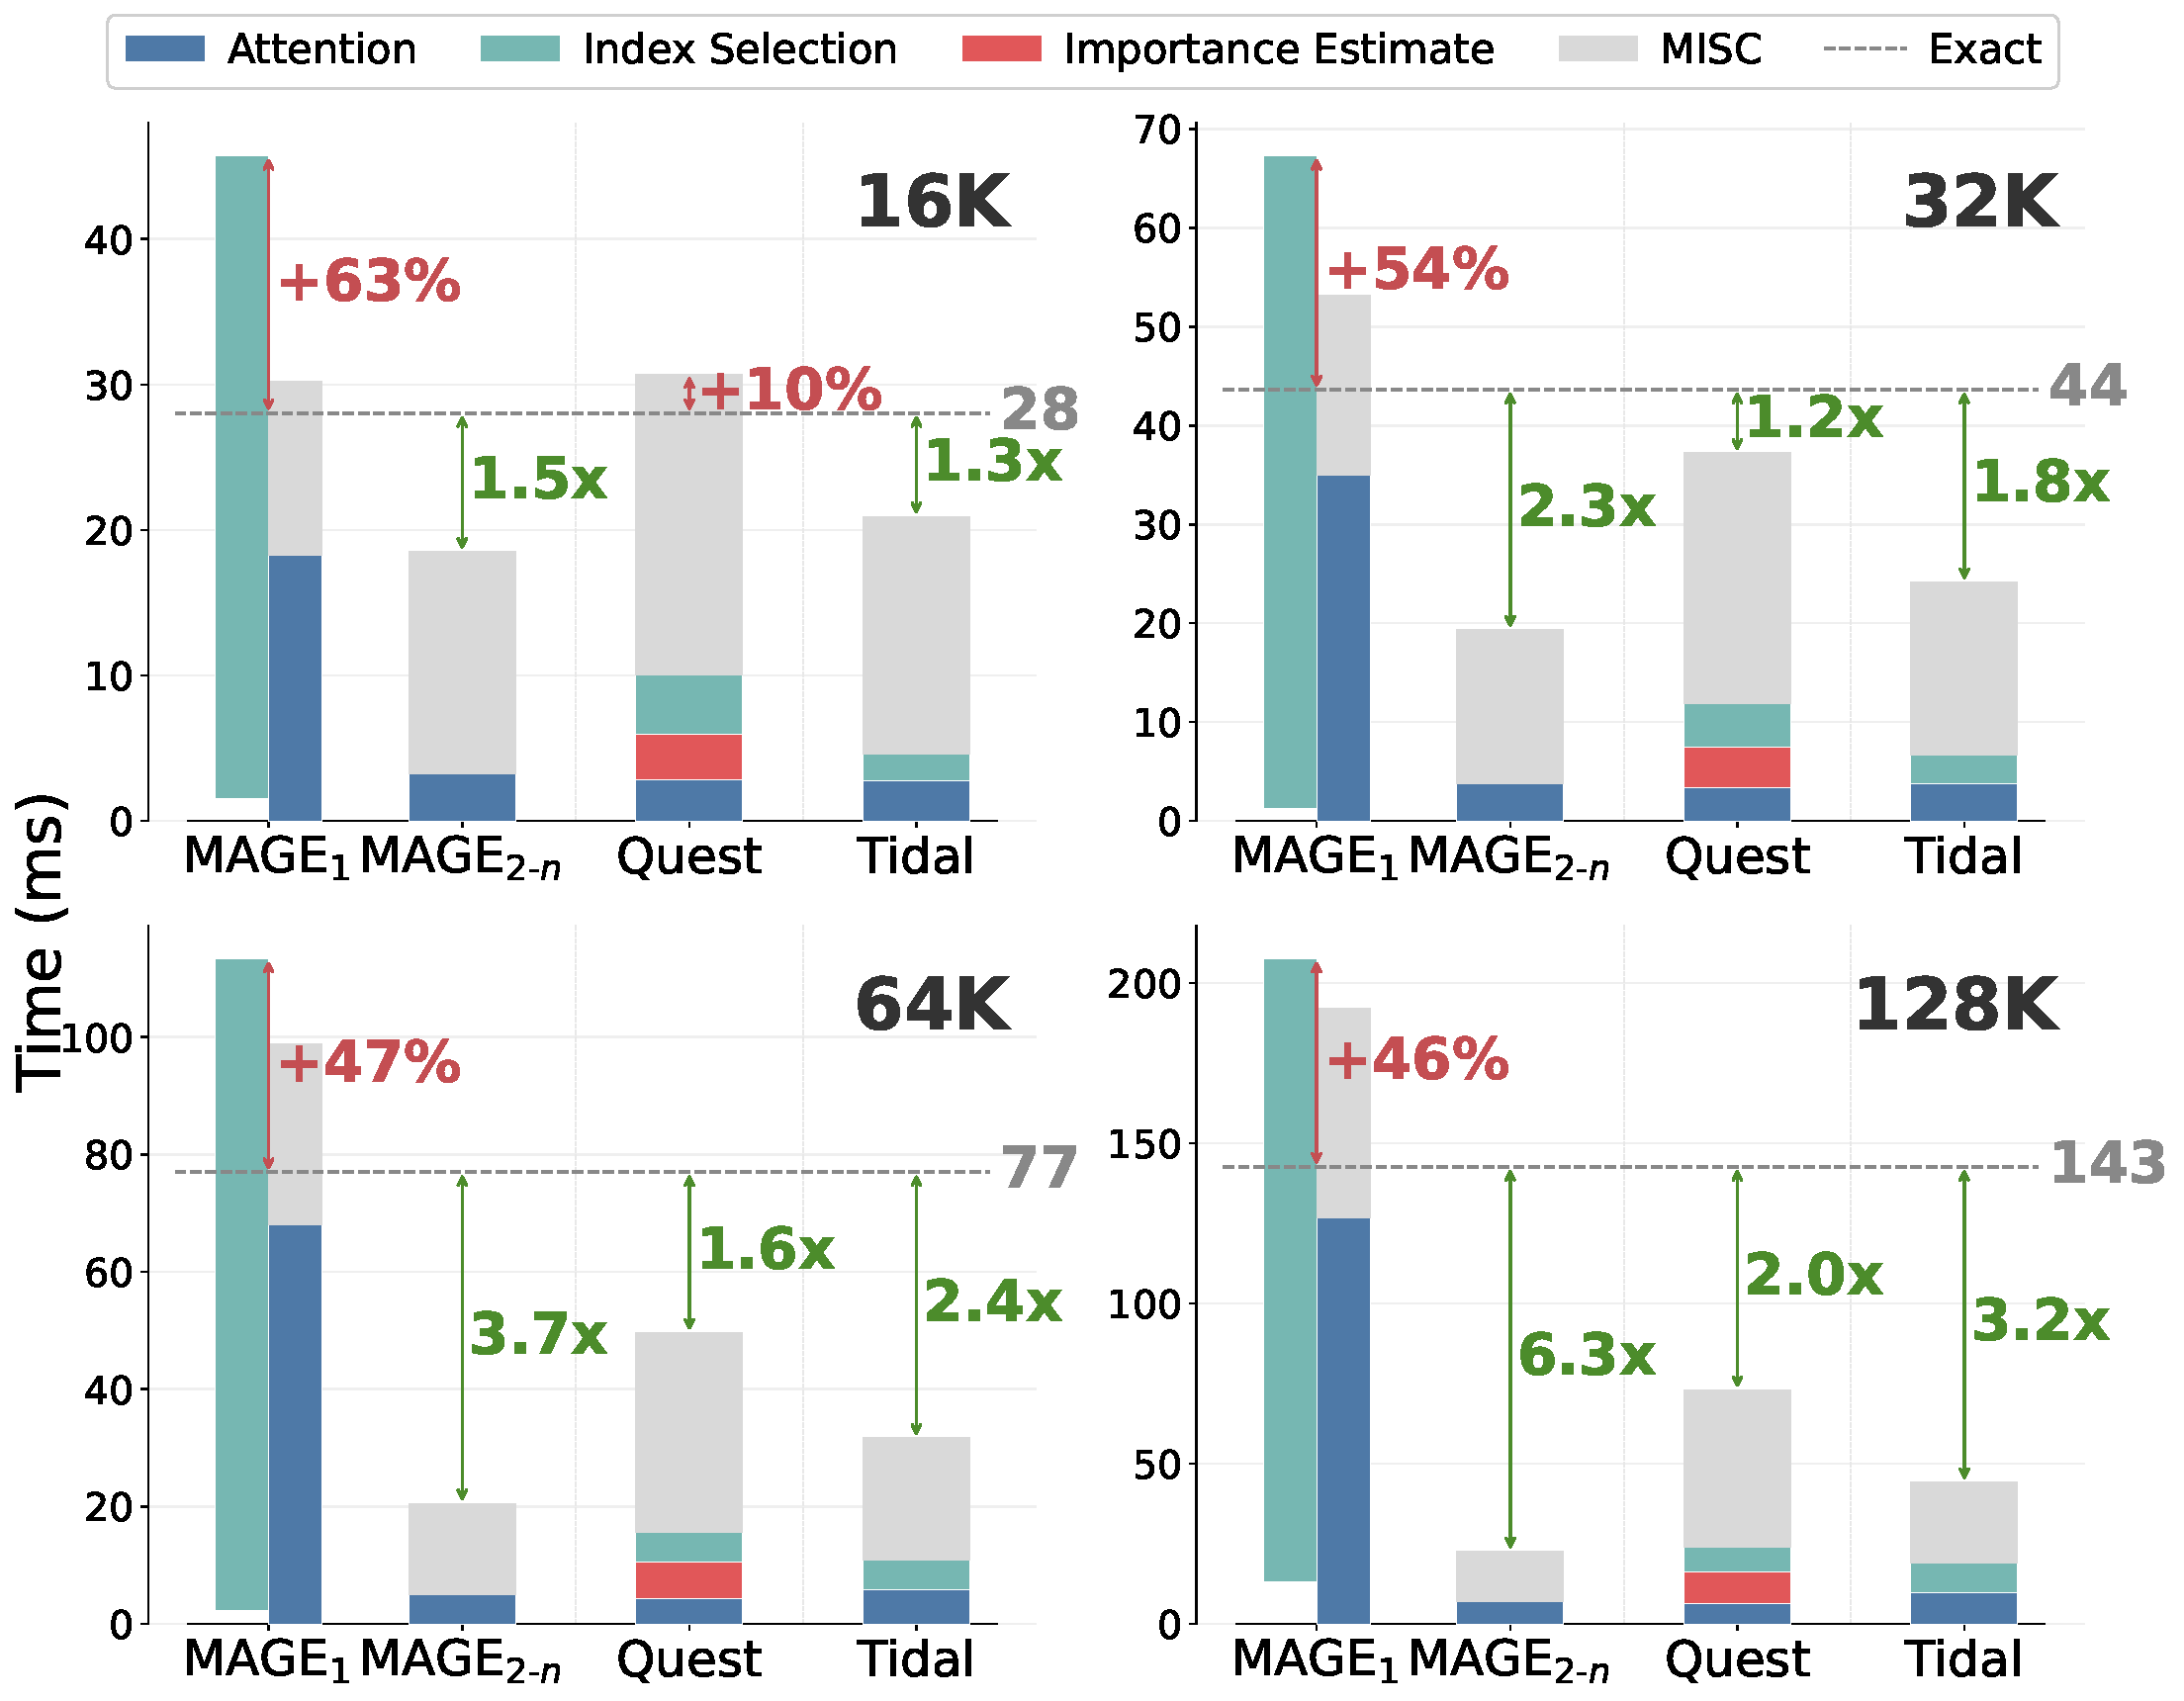
\includegraphics[width=\columnwidth]{figures/breakdown_small.pdf}
\caption{Denoising step latency breakdown from 16K to 128K context 
length (top-$k$=2048). For MAGE$_1$, stacked bars separate 
overlapped and main-stream operations. Dashed lines indicate 
exact attention latency. Extended results in Appendix~\ref{app:breakdown}.}
\label{fig:breakdown}
\end{figure}

\begin{figure}[t]
\centering
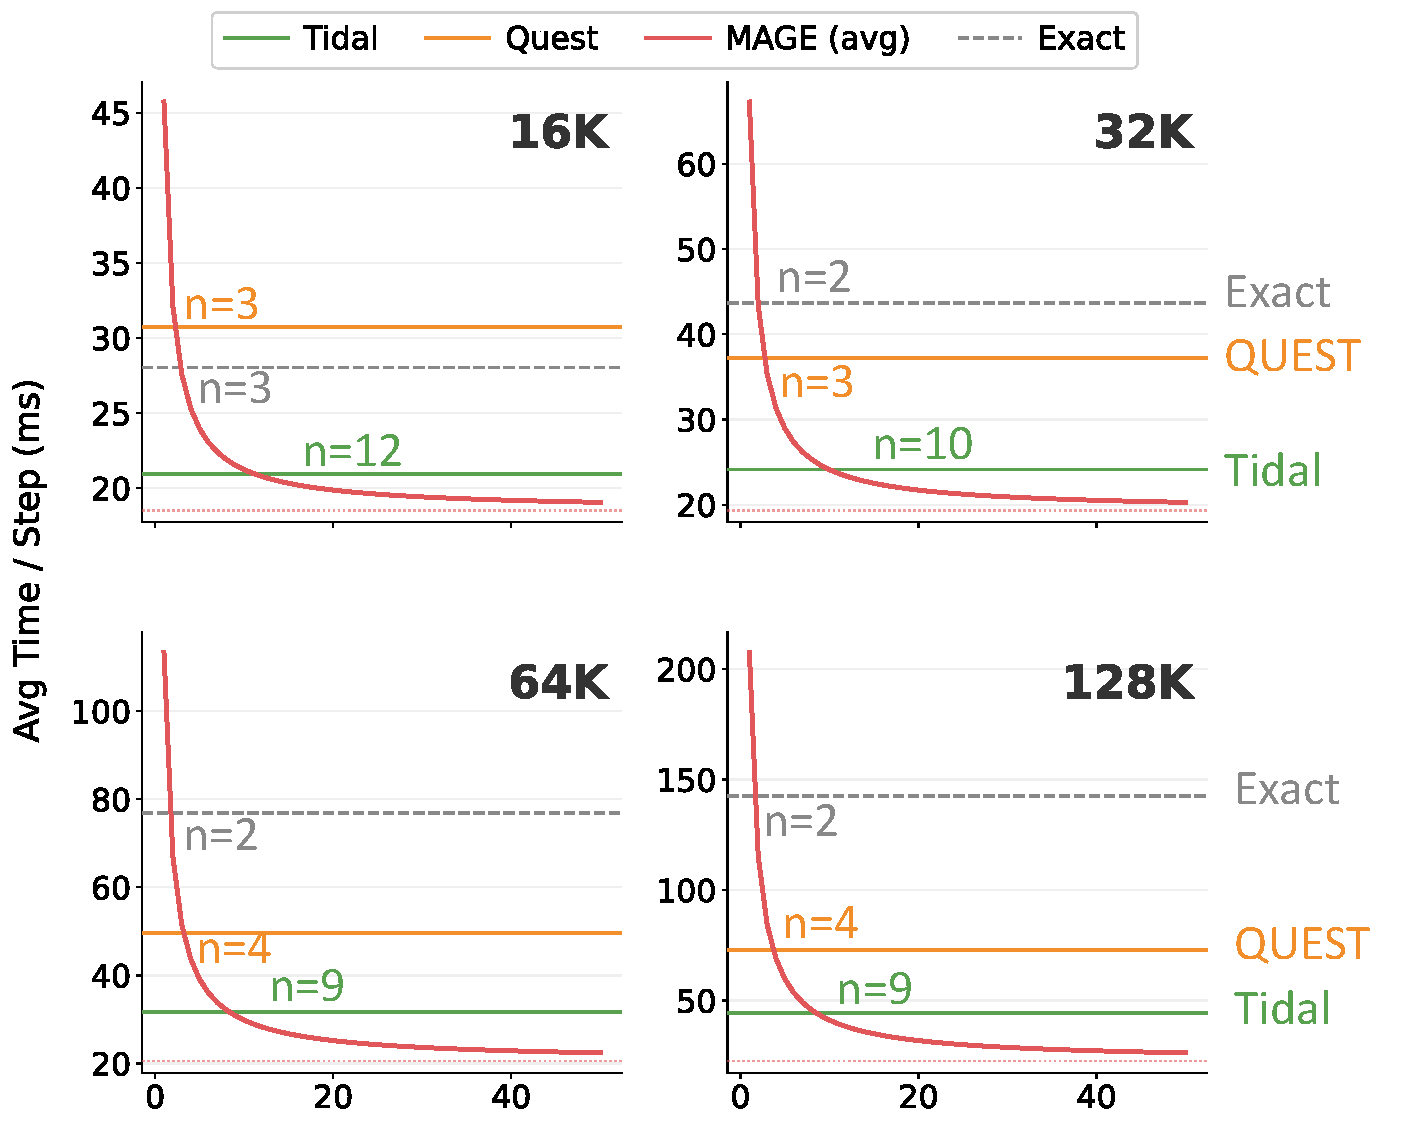
\includegraphics[width=\columnwidth]{figures/amortize_k2048.pdf}
\caption{Amortization of first-step overhead ($K$=2048). Dashed lines: baseline per-step latency. Labels: break-even step count.}
\label{fig:amortize}
\end{figure}



\paragraph{End to End Latency}



We evaluate the per-step inference latency of MAGE on LongBench (see Figure~\ref{fig:latency_1.5B}).
Per-step latency is defined as the total wall-clock time divided by the number of denoising steps, measured on a single GPU.
Compared with exact-attention decoding, MAGE yields substantial per-step speedups that scale with the number of tokens per step: on the 1.5B model, the average speedup increases from $1.66\times$ at $4\,$tokens/step to $2.01\times$ at $2\,$tokens/step and $2.37\times$ at $1\,$token/step;
on the 7B model, it grows from $1.48\times$ to $1.70\times$ and $1.81\times$ under the same settings, peaking at $3.92\times$ on NarrativeQA (1.5B, $1\,$token/step).
Among sparse attention baselines, MAGE consistently outperforms Quest in every pairwise comparison, achieving $1.48$--$2.15\times$ lower per-step latency on average.
Against Tidal, MAGE delivers competitive or superior latency at ${\leq}\,2\,$tokens/step, winning 75--79\% of comparisons at $1\,$token/step for both model sizes.
As illustrated in Figures~\ref{fig:longbench_accuracy} and \ref{fig:longbench_7b}, MAGE consistently outperforms other sparse attention methods in accuracy within the same computational budget, while maintaining highly competitive inference speeds.




\paragraph{Denoising Steps Breakdown}
Figure~\ref{fig:breakdown} shows the latency breakdown of a 
single denoising step across context lengths from 16K to 128K 
with top-$k$=2048. We classify all sparse index computation 
overhead, including importance estimation and top-$k$ filtering, 
under Index Selection. In the first denoising step (MAGE$_1$), 
our method incurs 46--63\% overhead compared to exact attention 
due to importance estimation, but multi-stream execution 
effectively overlaps this with attention computation. In 
subsequent steps (MAGE$_2$-$n$), our method achieves significant 
speedups: 1.5$\times$ at 16K, 2.3$\times$ at 32K, 3.7$\times$ 
at 64K, and 6.3$\times$ at 128K, consistently outperforming 
both Quest (1.1--2.0$\times$) and Tidal (1.3--3.2$\times$).
This scaling behavior is expected: as context length grows, 
the KV cache access becomes increasingly memory-bound, 
making the reduction from sparse attention more impactful.

\paragraph{Amortization of First-Step Overhead.}
As shown above, MAGE$_1$ incurs additional overhead due to 
exact attention for importance estimation. However, this 
cost is a one-time investment that benefits all subsequent 
denoising steps. Figure~\ref{fig:amortize} illustrates how 
this overhead is amortized as the number of denoising steps 
increases. The labels (e.g., $n$=9) denote the break-even 
point where MAGE becomes faster than each baseline. At 
shorter context lengths (16K), MAGE requires 12 steps to 
outperform Quest and 3 steps for Tidal. As context length 
increases, the break-even point decreases: at 128K, MAGE 
outperforms Tidal after only 2 steps and Quest after 4 steps. 
This trend arises because the first-step overhead ratio 
decreases with context length (from 63\% at 16K to 46\% 
at 128K), while per-step sparse savings scale proportionally. 
As a result, the break-even point drops to as few as 2 steps, 
and the overhead is amortized well within a single block's 
denoising process.

